\section{Trigonometric Integrals}
\begin{itemize}
    \item The first type of integral we'll deal with is:
    \begin{equation}
        \int \sin^nx\cos^nx \dd{x}
    \end{equation}
    \item In \textbf{case 1}, we have either $m$ or $n$ as an odd positive number. We can then use the identity $\sin^2x+\cos^2x=1$ to simplify it.
    \begin{example}
        For example, to solve $\int \sin^3 x \cos^2 x \dd{x}$, we can simplify this to:
        \begin{align}
            &= \int (1-\cos^2x)\cos^2 x \sin x \dd{X} \\ 
            &= (\cos^2x-\cos^4 x)\sin x \dd{x}
        \end{align}
        and applying a $u$ substitution with $u=\cos x$ and breaking it up into two integrals, we can get:
        \begin{equation}
            =-\frac{1}{3}\cos^3 x + \frac{1}{5}\cos^5 x + C
        \end{equation}
    \end{example}
    \item In \textbf{case 2}, we have $m$ and $n$ as both even. We then apply the double angle formulas:
    \begin{align}
        \sin x\cos x &= \frac{1}{2}\sin(2x) \\ 
        \sin^2 x &= \frac{1}{2} - \frac{1}{2}\cos 2x \\ 
        \cos^2 x &= \frac{1}{2} + \frac{1}{2}\cos 2x
    \end{align}
    \begin{example}
        For example:
        \begin{align}
            \int \sin^2 x\cos^4 \dd{x} &= \int \frac{1}{4}\sin^2(2x)\left(\frac{1}{2}+\frac{1}{2}\cos 2x\right) \dd{x} \\ 
            &= \frac{1}{8} \int \sin^2(2x) \dd{x} + \frac{1}{8}\int \sin^2 x\cos 2x \dd{x} \\ 
            &= \frac{1}{8} \int \left(\frac{1}{2} - \frac{1}{2}\cos 4x\right) \dd{x} + \frac{1}{8 \cdot 3 \cdot 2} \sin^3(2x) + C \\
            &= \frac{1}{16}x - \frac{1}{64}\sin(4x) + \frac{1}{48}\sin^3(2x) + C 
        \end{align}
    \end{example}
    \item In \textbf{Case 3}, we have:
    \begin{equation}
        \int \sin^n \dd{x},\, \int \cos^n \dd{x}
    \end{equation}
    which we can apply a reduction formula by keep applying integration by parts:
    \begin{align}
        \int \sin^n \dd{x} &= -\frac{1}{n}\sin^{n-1}x \cos x + \frac{n-1}{n} \int \sin^{n-2}x \dd{x} \\ 
        \int \cos^n \dd{x} &= \frac{1}{n}\cos^{n-1}x\sin x + \frac{n-1}{n}\int \cos^{n-2}x \dd{x}
    \end{align}
    \begin{example}
        To solve the integral $\int \sin^2 x \dd{x}$, we get:
        \begin{align}
            &= -\frac{1}{2}\sin x\cos x + \frac{1}{2} \int \dd{x} \\ 
            &= \frac{1}{2}x - \frac{1}{4}\sin 2x + C
        \end{align}
    \end{example}
    \item In \textbf{Case 4}, we have integrals in the following forms:
    \begin{align}
        &\int \sin(mx) \cos(nx) \dd{x} \\ 
        &\int \sin(mx) \sin(nx) \dd{x} \\ 
        &\int \cos(mx) \cos(nx) \dd{x}
    \end{align}
    with $m\neq n$. If $m=n$, then we can apply the double angle formula. To solve these, we apply the following identities:
    \begin{align}
        \sin A \sin B &= \frac{1}{2}\left[\cos(A-B) - \cos(A+B)\right] \\ 
        \cos A \cos B &= \frac{1}{2}\left[\cos(A-B) + \cos(A+B)\right] \\ 
        \sin A \cos B &= \frac{1}{2}\left[\sin(A-B) + \sin(A+B)\right]
    \end{align}
    \begin{example}
        For example, we have:
        \begin{align}
            \int \sin(3x)\sin(2x) \dd{x} &= \frac{1}{2} \int \cos((3-2)x) \dd{x} - \frac{1}{2}\cos((3+2)x) \dd{x} \\ 
            &= \frac{1}{2}\sin x - \frac{1}{10}\sin 5x + C
        \end{align}
    \end{example}
    \item In \textbf{case 5}, we have integrals in the form of either:
    \begin{equation}
        \int \tan^n x \dd{x},\, \int \cot^n x \dd{x}
    \end{equation}
    To solve these, we apply the following identities:
    \begin{align}
        \tan^2 x &= \sec^2 x - 1 \\ 
        & (\tan x)' = \sec^2 x 
    \end{align}
    \item In \textbf{case 6}, we have:
    \begin{equation}
        \int \sec^n x \dd{x},\, \int \csc^n x \dd{x}
    \end{equation}
    with $n \ge 2$. To solve these, we can make the following substitutions:
    \begin{align}
        1 + \tan^2 x &= \sec^2 x \\ 
        1 + \cot^2 x &= \csc^2 x
    \end{align}
    to convert it to a case 5 problem.
    \item In \textbf{case 7}, we have:
    \begin{equation}
        \int \tan^n x \sec^n x\dd{x},\, \int \cot^n x\csc^n x \dd{x}
    \end{equation}
    \begin{example}
        We have:
        \begin{align}
            \tan^3 x \sec^4 x \dd{x} &= \int \tan^3 x \sec^2 x \sec^2 x \dd{x} \\ 
            &= \int \tan^3 x\left(\tan^2 x + 1\right)\sec^2 x \dd{X} \\ 
            &= \int (\tan^5 x + \tan^3 x)\sec^2 x \dd{x} \\ 
            &= \frac{1}{6}\tan^6 x + \frac{1}{4}\tan^4 x + C
        \end{align}
    \end{example}
    \begin{idea}
        The basic idea of these types is to apply trigonometric identities to turn the integrals into a form that is easier to deal with. The substitutions are usually very simple but to find them, it requires a lot of practice.
    \end{idea}
    \item We can also apply \textbf{trigonometric substitutions}, any integrals with any of the three factors below can be solved with this technique:
    \begin{enumerate}
        \item $\sqrt{a^2-x^2}$: Set $x=a\sin u \implies \sqrt{a^2-x^2} = a\cos u$
        \item $\sqrt{a^2+x^2}$: Set $x=a\tan u \implies \sqrt{a^2+x^2}=a\sec u$
        \item $\sqrt{x^2-a^2}$: Set $x=a\sec u \implies \sqrt{x^2-a^2} = a\tan u$
    \end{enumerate}
    where the arguments under the square roots are always positive.
    \begin{example}
        To solve the integral $\int \frac{x^2}{(4-x^2)^{3/2}} \dd{x}$, we can set:
        \begin{align}
            x &= 2\sin u \\ 
            \dd{x} &= 2\cos u \dd{u} \\ 
            \sqrt{4-x^2} &= 2\cos u
        \end{align}
        which gives:
        \begin{align}
            &= \int \frac{4\sin^2 u \cdot 2\cos u \dd{u}}{8\cos^3 u} \\ 
            &= \int \tan^2 u \dd{u} \\ 
            &= \int (\sec^2 u -1) \dd{u} \\ 
            &= \tan u - u + C
            &= \frac{x}{\sqrt{4-x^2}} - \sin^{-1}\left(\frac{x}{2}\right)+C
        \end{align}
    \end{example}
    \begin{example}
        The integral $\int \frac{x \dd{x}}{(2x^2+4x-7)^{1/2}}$ needs a bit more work before we can apply the sibstutitions. We first apply the square to get:
        \begin{equation}
            = \int \frac{x \dd{x}}{\sqrt{2(x+1)^2 - 9}}
        \end{equation}
        We can set:
        \begin{align}
            \sqrt{2} (x+1) &= 3\sec u \\ 
            \sqrt{2} \dd{x} &= 3\sec u \tan u \dd{u} \\ 
            \sqrt{2(x+1)^2-9} &= 3\tan u
        \end{align}
        which gives:
        \begin{align}
            &= \int \frac{\left(\frac{3}{\sqrt{2}}\sec u - 1\right)\left(\frac{3}{\sqrt{2}\sec u \tan u \dd{u}}\right)}{3\tan u} \\ 
            &= \int \left(\frac{3}{\sqrt{2}}\sec u -1\right)\left(\frac{1}{\sqrt{2}}\sec u\right) \dd{u} \\ 
            &= \frac{3}{2}\int \sec^2 u \dd{u} - \frac{1}{\sqrt{2}}\int \sec u \dd{u} \\ 
            &= \frac{3}{2}\tan u - \frac{1}{\sqrt{2}}\ln|\sec u + \tan u| + C \\
            &= \frac{1}{2}\sqrt{2x^2+4x-7} - \frac{1}{\sqrt{2}}\ln\left|\frac{\sqrt{2}}{3}(x+1)+\frac{\sqrt{2x^2+4x-7}}{3}\right| + C
        \end{align}
    \end{example}
    \begin{idea}
        We can use triangles to derive the substitution, which comes from the Pythagorean theorem:
        \begin{center}
            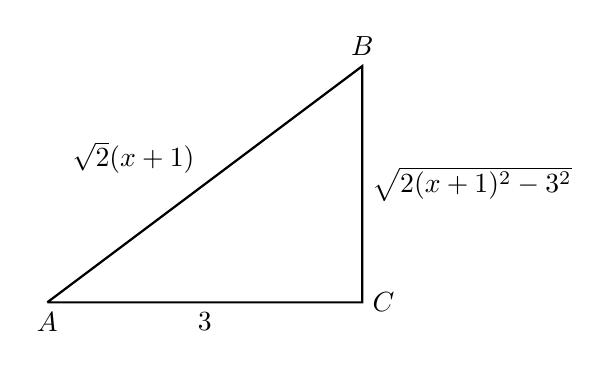
\begin{tikzpicture}
                \draw[thick] (0,0) node[below] {$A$} -- node[midway,above left] {$\sqrt{2}(x+1)$} (4,3) node[above] {$B$} -- node[midway,right] {$\sqrt{2(x+1)^2-3^2}$} (4,0) node[right] {$C$} -- node[midway,below] {$3$} (0,0);
            \end{tikzpicture}
        \end{center}
        and you can clearly see the substitution:
        \begin{equation}
            3\sec u = \sqrt{2}(x+1) \implies \cos u = \frac{3}{\sqrt{2} (x+1)}
        \end{equation}
        where $u \equiv \angle BAC$.
    \end{idea}
    \begin{example}
        For the integral $\int x \sin^{-1} x \dd{x}$, we can let:
        \begin{align}
            u = \sin^{-1} x & \dd{v} = x \dd{x} \\
            \dd{u} = \frac{\dd{x}}{\sqrt{1-x^2}} & v = \frac{1}{2}x^2 
        \end{align}
        and applying integration by parts, we get:
        \begin{align}
            =\frac{1}{2}x^2 \sin^{-1} x - \int \frac{1}{2}x^2 \frac{\dd{x}}{\sqrt{1-x^2}}
        \end{align}
        To solve this secondary integral $\int \frac{x^2 \dd{x}}{\sqrt{1-x^2}}$, we can let:
        \begin{align}
            x &= \sin\theta \\ 
            \dd{x} &= \cos \theta \dd{\theta} \\ 
            \sqrt{1-x^2} &= \cos\theta 
        \end{align}
        which gives:
        \begin{align}
            &= \frac{\sin^2 \theta \cos\theta \dd{\theta}}{\cos\theta} \\ 
            &= \int \sin^2 \theta \dd{\theta} \\ 
            &= \frac{1}{2}\theta - \frac{1}{2}\sin\theta\cos\theta + C \\ 
            &= \frac{1}{2}\sin^{-1} - \frac{1}{2}x\sqrt{1-x^2} + C
        \end{align}
        Therefore, we get:
        \begin{equation}
            \int x\sin^{-1} x \dd{x} = \frac{1}{2}x^2\sin^{-1}x - \frac{1}{4}\sin^{-1} x + \frac{1}{4} x \sqrt{1-x^2} + C
        \end{equation}
    \end{example}
\end{itemize}